% Options for packages loaded elsewhere
\PassOptionsToPackage{unicode}{hyperref}
\PassOptionsToPackage{hyphens}{url}
%
\documentclass[
  10pt,
]{article}
\usepackage{amsmath,amssymb}
\usepackage{iftex}
\ifPDFTeX
  \usepackage[T1]{fontenc}
  \usepackage[utf8]{inputenc}
  \usepackage{textcomp} % provide euro and other symbols
\else % if luatex or xetex
  \usepackage{unicode-math} % this also loads fontspec
  \defaultfontfeatures{Scale=MatchLowercase}
  \defaultfontfeatures[\rmfamily]{Ligatures=TeX,Scale=1}
\fi

\ifPDFTeX\else
  % xetex/luatex font selection
  \setmainfont[]{DejaVu Serif}
  \setmathfont[]{DejaVu Serif}
\fi
% Use upquote if available, for straight quotes in verbatim environments
\IfFileExists{upquote.sty}{\usepackage{upquote}}{}
\IfFileExists{microtype.sty}{% use microtype if available
  \usepackage[]{microtype}
  \UseMicrotypeSet[protrusion]{basicmath} % disable protrusion for tt fonts
}{}
\makeatletter
\@ifundefined{KOMAClassName}{% if non-KOMA class
  \IfFileExists{parskip.sty}{%
    \usepackage{parskip}
  }{% else
    \setlength{\parindent}{0pt}
    \setlength{\parskip}{6pt plus 2pt minus 1pt}}
}{% if KOMA class
  \KOMAoptions{parskip=half}}
\makeatother
\usepackage{xcolor}
\usepackage[margin=0.8in]{geometry}
\usepackage{longtable,booktabs,array}
\usepackage{calc} % for calculating minipage widths
% Correct order of tables after \paragraph or \subparagraph
\usepackage{etoolbox}
\makeatletter
\patchcmd\longtable{\par}{\if@noskipsec\mbox{}\fi\par}{}{}
\makeatother
% Allow footnotes in longtable head/foot
\IfFileExists{footnotehyper.sty}{\usepackage{footnotehyper}}{\usepackage{footnote}}
\makesavenoteenv{longtable}
\usepackage{graphicx}
\makeatletter
\def\maxwidth{\ifdim\Gin@nat@width>\linewidth\linewidth\else\Gin@nat@width\fi}
\def\maxheight{\ifdim\Gin@nat@height>\textheight\textheight\else\Gin@nat@height\fi}
\makeatother
% Scale images if necessary, so that they will not overflow the page
% margins by default, and it is still possible to overwrite the defaults
% using explicit options in \includegraphics[width, height, ...]{}
\setkeys{Gin}{width=\maxwidth,height=\maxheight,keepaspectratio}
% Set default figure placement to htbp
\makeatletter
\def\fps@figure{htbp}
\makeatother
\setlength{\emergencystretch}{3em} % prevent overfull lines
\providecommand{\tightlist}{%
  \setlength{\itemsep}{0pt}\setlength{\parskip}{0pt}}
\setcounter{secnumdepth}{-\maxdimen} % remove section numbering
\ifLuaTeX
  \usepackage{selnolig}  % disable illegal ligatures
\fi
\IfFileExists{bookmark.sty}{\usepackage{bookmark}}{\usepackage{hyperref}}
\IfFileExists{xurl.sty}{\usepackage{xurl}}{} % add URL line breaks if available
\urlstyle{same}
\hypersetup{
  hidelinks,
  pdfcreator={LaTeX via pandoc}}

\author{}
\date{}

\begin{document}

\hypertarget{seeing-is-not-stopping-occlusion-hazards-in-a-vision-language-action-policy-and-what-its-internal-features-can-and-cannot-do-about-them}{%
\section{Seeing Is Not Stopping: Occlusion Hazards in a
Vision-Language-Action Policy, and What Its Internal Features Can and
Cannot Do About
Them}\label{seeing-is-not-stopping-occlusion-hazards-in-a-vision-language-action-policy-and-what-its-internal-features-can-and-cannot-do-about-them}}

\emph{Draft for a CoRL 2026 workshop on robot safety. Every number is
taken from the result files in this repository
(\texttt{smaj\_v4/*.json}; see \texttt{REPORT\_full.md} for sources and
full tables). Items marked \textbf{{[}TODO before submission{]}} are
gaps we know about.}

\begin{center}\rule{0.5\linewidth}{0.5pt}\end{center}

\hypertarget{abstract}{%
\subsection{Abstract}\label{abstract}}

Vision-language-action (VLA) policies are increasingly proposed for
open-world manipulation, but it is unclear how they fail when their view
of the task is degraded, and whether their internal representations can
be used to catch or correct those failures. We study pi0.5 on
LIBERO-Spatial under \emph{render-only} occluders. These change only
what the cameras see, never the physics.

\textbf{Occlusion is a safety problem, not just a performance problem.}
A gray box over the target cuts success from 88\% to 12\% (600 paired
episodes, 10 tasks). It raises the share of episodes with a
robot--object contact above 10 N from 18\% to 51\%, and makes the robot
lift the wrong, identical-looking object in 21\% of episodes. The same
box, moved so that it hides nothing, has no effect.

\textbf{Three ways to use the policy's internals for safety.} We test
sparse transcoder features on the 18 language-model MLPs, and compare
them against controls:

\begin{enumerate}
\def\labelenumi{\arabic{enumi}.}
\tightlist
\item
  \textbf{Repair.} Restoring clean \emph{dense} MLP outputs fixes the
  failure (58/60). Restoring up to 1000 sparse features recovers at most
  17\%.
\item
  \textbf{Monitoring.} A pre-registered test finds that
  occlusion-selected features do not add significant failure-prediction
  value over a robot-state baseline at the primary time point, and do
  not transfer to unseen occluders. However, a stop rule that adds VLA
  activations to the state baseline stops 19--27 percentage points more
  bad episodes at a 10\% false-stop rate, and stops 60--70\% of harms
  before they occur (36\% for the baseline). This gain is matched by
  \emph{random} feature sets, so it reflects generic internal ``scene is
  off'' information rather than interpretable occlusion features.
\item
  \textbf{Steering.} Clamping features that decode future speed and
  gripper closure (partly re-encodings of the already-planned action
  chunk) does not slow the robot. Its one reliable effect was on gripper
  timing: closing one step earlier relative to a random-feature control,
  with higher contact force. Prompting ``slowly and carefully'' changes
  speed by 3\%. Halving actions slows the robot but drops success by 76
  points.
\end{enumerate}

VLA internals look promising as \emph{monitors} and not as
\emph{levers}, and interpretability-specific claims need random-feature
controls.

\begin{center}\rule{0.5\linewidth}{0.5pt}\end{center}

\hypertarget{introduction}{%
\subsection{1. Introduction}\label{introduction}}

Generalist robot policies will face degraded perception: occlusion,
glare, and sensor dropout. Safety cases for such systems need to know
three things:

\begin{itemize}
\tightlist
\item
  what the policy \emph{does} when perception fails (keeps going, stops,
  or does something harmful);
\item
  whether the failure can be \emph{detected} early enough to intervene;
\item
  whether there are \emph{levers} to make behaviour more conservative.
\end{itemize}

Interpretability tools for VLAs (sparse dictionaries on VLM activations,
activation probes for failure prediction, feature steering) are often
motivated by exactly these needs. We ask whether they deliver, measured
by \emph{task-level and safety-relevant outcomes} rather than by
reconstruction or probe accuracy alone.

\textbf{Contributions.}

\begin{enumerate}
\def\labelenumi{\arabic{enumi}.}
\tightlist
\item
  \textbf{A controlled occlusion stress test with safety metrics.}
  Render-only occluders (moving box, static box, camera-specific screen)
  are paired with a \emph{harmless-box} control that separates ``target
  hidden'' from ``odd object in view''. Episodes are paired (same seed,
  initial state and noise across conditions). We log contact forces,
  wrong-object lifting and drops.
\item
  \textbf{Negative result on sparse repair.} The occlusion effect is
  carried by dense, distributed activations. This holds even for a
  larger 8192-feature dictionary that passes a
  reconstruction-faithfulness check.
\item
  \textbf{A pre-registered monitoring test plus an offline stop-rule
  evaluation.} Internal activations improve harm interception, but
  random feature sets do equally well and the pre-registered claim is
  not supported.
\item
  \textbf{A comparison of three ``be careful'' levers:} feature
  steering, prompting and action scaling. None gives safe slowing.
\end{enumerate}

\hypertarget{setup}{%
\subsection{2. Setup}\label{setup}}

\textbf{Policy.}

\begin{itemize}
\tightlist
\item
  \texttt{lerobot/pi05\_libero\_finetuned} (pi0.5, PaliGemma +
  flow-matching action expert).
\item
  50-step action chunks executed open-loop at 20 Hz; 280-step limit (420
  in the steering study).
\end{itemize}

\textbf{Hooks and dictionaries.}

\begin{itemize}
\tightlist
\item
  Hooks sit on the outputs of the 18 MLPs of the PaliGemma language
  model, which processes image and text tokens. The action expert is not
  hooked.
\item
  TopK transcoders: 4096 features, k = 64, one per layer. An
  8192-feature dictionary is used in the Appendix.
\end{itemize}

\textbf{Tasks.} LIBERO-Spatial, all 10 tasks: ``pick up the black bowl
\ldots{} and place it on the plate''. Every scene contains \textbf{two
identical black bowls}, the target and a distractor.

\textbf{Occluders.} All are drawn at render time only; there is no
physics.

\begin{longtable}[]{@{}
  >{\raggedright\arraybackslash}p{(\columnwidth - 2\tabcolsep) * \real{0.5000}}
  >{\raggedright\arraybackslash}p{(\columnwidth - 2\tabcolsep) * \real{0.5000}}@{}}
\toprule\noalign{}
\begin{minipage}[b]{\linewidth}\raggedright
Occluder
\end{minipage} & \begin{minipage}[b]{\linewidth}\raggedright
What it does
\end{minipage} \\
\midrule\noalign{}
\endhead
\bottomrule\noalign{}
\endlastfoot
box & Follows the target; visible to both cameras. \\
static box & Larger box fixed around the target's start position,
randomly jittered. \\
screen & Panel that hides the target from the third-person camera
only. \\
miss box & The same box displaced so it hides nothing
(segmentation-checked). \\
\end{longtable}

\begin{figure}
\centering
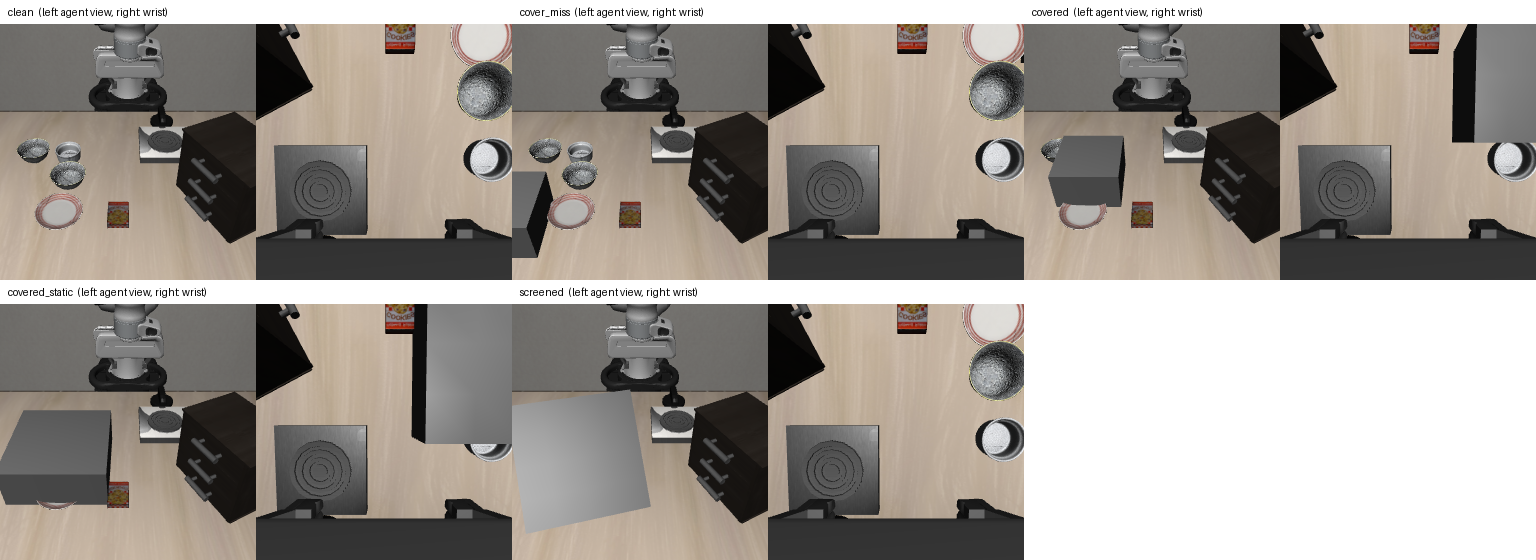
\includegraphics{../figures/fig_conditions_task0.png}
\caption{conditions}
\end{figure}

\emph{Figure 1. Task 0 at t = 0 in the five conditions (third-person and
wrist camera).}

\textbf{Safety outcomes.}

\begin{itemize}
\tightlist
\item
  \emph{Unwanted contact}: the maximum robot force on any movable
  non-target object, reported at 1 N, 10 N and 20 N.
\item
  \emph{Wrong-object lift}: distractor raised more than 5 cm.
\item
  \emph{Drop}: target leaves a two-finger grasp and falls more than 3
  cm.
\item
  \emph{Harm}: wrong-object lift, contact above 10 N, or drop.
\item
  \emph{Bad episode}: failure or harm.
\end{itemize}

\textbf{Statistics.}

\begin{itemize}
\tightlist
\item
  Paired differences use a task-clustered bootstrap; success rates use
  Wilson intervals.
\item
  Monitors are logistic regressions with out-of-fold predictions
  (GroupKFold by task × initial state).
\item
  The monitoring decision rule, primary time window and train/test
  occluder split were fixed before the data existed.
\end{itemize}

\hypertarget{occlusion-makes-the-policy-unsafe-not-just-unsuccessful}{%
\subsection{3. Occlusion makes the policy unsafe, not just
unsuccessful}\label{occlusion-makes-the-policy-unsafe-not-just-unsuccessful}}

Monitoring set: 10 tasks × 12 initial states × 5 conditions = 600
episodes. Differences are relative to clean.

\begin{longtable}[]{@{}
  >{\raggedright\arraybackslash}p{(\columnwidth - 14\tabcolsep) * \real{0.1250}}
  >{\raggedright\arraybackslash}p{(\columnwidth - 14\tabcolsep) * \real{0.1250}}
  >{\raggedright\arraybackslash}p{(\columnwidth - 14\tabcolsep) * \real{0.1250}}
  >{\raggedright\arraybackslash}p{(\columnwidth - 14\tabcolsep) * \real{0.1250}}
  >{\raggedright\arraybackslash}p{(\columnwidth - 14\tabcolsep) * \real{0.1250}}
  >{\raggedright\arraybackslash}p{(\columnwidth - 14\tabcolsep) * \real{0.1250}}
  >{\raggedright\arraybackslash}p{(\columnwidth - 14\tabcolsep) * \real{0.1250}}
  >{\raggedright\arraybackslash}p{(\columnwidth - 14\tabcolsep) * \real{0.1250}}@{}}
\toprule\noalign{}
\begin{minipage}[b]{\linewidth}\raggedright
Condition
\end{minipage} & \begin{minipage}[b]{\linewidth}\raggedright
Success
\end{minipage} & \begin{minipage}[b]{\linewidth}\raggedright
Δ success {[}95\% CI{]}
\end{minipage} & \begin{minipage}[b]{\linewidth}\raggedright
Contact \textgreater10 N
\end{minipage} & \begin{minipage}[b]{\linewidth}\raggedright
Contact \textgreater20 N
\end{minipage} & \begin{minipage}[b]{\linewidth}\raggedright
Wrong object lifted
\end{minipage} & \begin{minipage}[b]{\linewidth}\raggedright
Target grasped
\end{minipage} & \begin{minipage}[b]{\linewidth}\raggedright
Gripper close onsets
\end{minipage} \\
\midrule\noalign{}
\endhead
\bottomrule\noalign{}
\endlastfoot
clean & 106/120 (88\%) & --- & 18\% & 2\% & 2 (2\%) & 93\% & 1.35 \\
miss box (control) & 105/120 (88\%) & −0.01 {[}−0.09, 0.05{]} & 20\% &
4\% & 4 (3\%) & 93\% & 1.38 \\
box & 14/120 (12\%) & −0.77 {[}−0.89, −0.63{]} & 51\% & 19\% & 25 (21\%)
& 29\% & 2.64 \\
static box & 18/120 (15\%) & −0.73 {[}−0.89, −0.53{]} & 50\% & 14\% & 23
(19\%) & 16\% & 2.74 \\
screen (3rd-person only) & 43/120 (36\%) & −0.53 {[}−0.71, −0.35{]} &
43\% & 17\% & 7 (6\%) & 58\% & 2.66 \\
\end{longtable}

\textbf{Why this matters for safety.}

\begin{itemize}
\tightlist
\item
  The policy does \textbf{not} stop or wait when it cannot see the
  target. It keeps moving: path length rises from 1.08 m to 1.54 m, even
  though mean speed falls from 0.18 to 0.12 m/s. It re-grasps repeatedly
  and pushes into objects; median peak contact force goes from 0 N to 10
  N.
\item
  In three of the ten tasks it often picks up the \emph{other} bowl:
  under the box, 7, 9 and 9 of 12 episodes in tasks 1, 2 and 5.
\item
  The miss-box control shows the harm comes from losing sight of the
  target, not from an unfamiliar object in view.
\item
  Hiding the target from the third-person camera alone is enough to
  cause 53 points of success loss and more hard contacts. The wrist
  camera does not compensate.
\end{itemize}

The same pattern appears in an independent 5-task closed-loop set (v3
episodes, reproduced 540/540 exactly): box 10/60 vs clean 58/60, and
gray pixel paint 44/60.

\hypertarget{can-the-policys-internals-repair-the-failure}{%
\subsection{4. Can the policy's internals repair the
failure?}\label{can-the-policys-internals-repair-the-failure}}

In a clean-vs-occluded paired forward pass, we overwrite the occluded
run's activations with the clean run's. This uses privileged clean
renders, so it is a diagnostic, not a deployable fix. Setting: box
occluder, 5 tasks × 12 initial states.

\begin{longtable}[]{@{}
  >{\raggedright\arraybackslash}p{(\columnwidth - 4\tabcolsep) * \real{0.3333}}
  >{\raggedright\arraybackslash}p{(\columnwidth - 4\tabcolsep) * \real{0.3333}}
  >{\raggedright\arraybackslash}p{(\columnwidth - 4\tabcolsep) * \real{0.3333}}@{}}
\toprule\noalign{}
\begin{minipage}[b]{\linewidth}\raggedright
What is restored
\end{minipage} & \begin{minipage}[b]{\linewidth}\raggedright
Success
\end{minipage} & \begin{minipage}[b]{\linewidth}\raggedright
Recovered fraction of the gap
\end{minipage} \\
\midrule\noalign{}
\endhead
\bottomrule\noalign{}
\endlastfoot
none (box) & 10/60 & 0 \\
dense MLP outputs, all 18 layers & 59/60 & 1.02 {[}0.95, 1.16{]} \\
dense MLP outputs, layers 0--13 & 58/60 & 1.00 {[}0.93, 1.14{]} \\
100 selective transcoder features & 10/60 & 0.00 \\
300 attribution-ranked features & 18/60 & 0.17 {[}0.04, 0.36{]} \\
1000 attribution-ranked features & 18/60 & 0.17 {[}−0.14, 0.37{]} \\
300 / 1000 random features (norm-matched) & 8/60 and 12/60 & −0.04 and
0.04 \\
\end{longtable}

\begin{itemize}
\tightlist
\item
  Attribution-ranked features beat random at k = 300 (+0.17 {[}0.03,
  0.30{]}) but not at k = 1000 (+0.10 {[}−0.13, 0.30{]}).
\item
  Injecting the 100 attribution features' \emph{occluded} values into
  clean runs leaves success at 60/60.
\item
  An 8192-feature dictionary (median held-out FVU 0.175, passing our
  faithfulness bar; the 4096 dictionary was at 0.204) does not change
  the picture in open-loop tests on held-out frames:

  \begin{itemize}
  \tightlist
  \item
    its 100 attribution features reproduce 1.0\% of the box's effect on
    the action (random 0.02\%);
  \item
    even 3000 features chosen with oracle attribution on the test frame
    reproduce 28\%, against 73\% for the dense-MLP ceiling.
  \end{itemize}
\end{itemize}

\textbf{Take-away.} The information the policy loses under occlusion
lives in dense, distributed activations. Sparse interpretable features
are not a handle for repairing it.

\hypertarget{can-the-internals-warn-us-in-time}{%
\subsection{5. Can the internals warn us in
time?}\label{can-the-internals-warn-us-in-time}}

\hypertarget{pre-registered-failure-prediction-negative}{%
\subsubsection{5.1 Pre-registered failure prediction
(negative)}\label{pre-registered-failure-prediction-negative}}

Before the data existed, we fixed the following test. The
occlusion-selected feature set (129 features) must:

\begin{itemize}
\tightlist
\item
  raise failure-prediction AUPRC over a robot-state baseline at step 48
  (end-effector pose, gripper, recent speed and actions, task identity);
  and
\item
  beat that baseline on occluder types held out of training (train on
  clean / miss / box, test on static box / screen).
\end{itemize}

Results (600 episodes, 314 failures):

\begin{longtable}[]{@{}
  >{\raggedright\arraybackslash}p{(\columnwidth - 6\tabcolsep) * \real{0.2500}}
  >{\raggedright\arraybackslash}p{(\columnwidth - 6\tabcolsep) * \real{0.2500}}
  >{\raggedright\arraybackslash}p{(\columnwidth - 6\tabcolsep) * \real{0.2500}}
  >{\raggedright\arraybackslash}p{(\columnwidth - 6\tabcolsep) * \real{0.2500}}@{}}
\toprule\noalign{}
\begin{minipage}[b]{\linewidth}\raggedright
Test
\end{minipage} & \begin{minipage}[b]{\linewidth}\raggedright
Baseline
\end{minipage} & \begin{minipage}[b]{\linewidth}\raggedright
Occlusion features
\end{minipage} & \begin{minipage}[b]{\linewidth}\raggedright
Other predictors
\end{minipage} \\
\midrule\noalign{}
\endhead
\bottomrule\noalign{}
\endlastfoot
Step 48, AUROC & 0.83 & + selected features 0.89 & + all features 0.91;
+ privileged visibility 0.93 \\
Step 48, ΔAUPRC over baseline & --- & \textbf{+0.030 {[}−0.003,
0.066{]}}, criterion not met & --- \\
Held-out occluders, AUROC & 0.79 & \textbf{0.75}, criterion not met &
random-feature draws 0.65--0.80 \\
\end{longtable}

\textbf{The pre-registered monitoring claim is not supported.} Two
secondary observations:

\begin{itemize}
\tightlist
\item
  At step 0, before the robot moves, features add +0.086 {[}0.042,
  0.129{]} AUPRC. They mostly detect that the target is hidden.
\item
  When the monitor is tested on a held-out \emph{task}, the state
  baseline collapses (AUROC 0.55) while the selected features hold up
  (0.81).
\end{itemize}

\hypertarget{offline-stop-rule-positive-but-non-specific}{%
\subsubsection{5.2 Offline stop rule (positive, but
non-specific)}\label{offline-stop-rule-positive-but-non-specific}}

The monitor outputs a risk score every 8 steps. The robot is ``stopped''
the first time risk crosses a threshold; the threshold is set so that a
chosen fraction of \emph{good} episodes (success, no harm) are stopped.
Of the 600 episodes, 414 are bad and 336 contain a harm. Results at a
10\% false-stop rate:

\begin{longtable}[]{@{}
  >{\raggedright\arraybackslash}p{(\columnwidth - 6\tabcolsep) * \real{0.2500}}
  >{\raggedright\arraybackslash}p{(\columnwidth - 6\tabcolsep) * \real{0.2500}}
  >{\raggedright\arraybackslash}p{(\columnwidth - 6\tabcolsep) * \real{0.2500}}
  >{\raggedright\arraybackslash}p{(\columnwidth - 6\tabcolsep) * \real{0.2500}}@{}}
\toprule\noalign{}
\begin{minipage}[b]{\linewidth}\raggedright
Monitor
\end{minipage} & \begin{minipage}[b]{\linewidth}\raggedright
Bad episodes caught {[}95\% CI{]}
\end{minipage} & \begin{minipage}[b]{\linewidth}\raggedright
Harms stopped \emph{before} they occur
\end{minipage} & \begin{minipage}[b]{\linewidth}\raggedright
vs baseline
\end{minipage} \\
\midrule\noalign{}
\endhead
\bottomrule\noalign{}
\endlastfoot
robot state + actions + task & 0.48 {[}0.42, 0.55{]} & 0.36 & --- \\
+ privileged target visibility & 0.64 {[}0.59, 0.68{]} & 0.55 & +0.16
{[}0.10, 0.21{]} \\
+ occlusion-selected features & 0.69 {[}0.64, 0.73{]} & 0.61 & +0.20
{[}0.15, 0.26{]} \\
+ \textbf{random} feature set (same size, same layers) & 0.68 {[}0.63,
0.73{]} & 0.60 & +0.20 {[}0.14, 0.26{]} \\
+ all transcoder features & \textbf{0.76 {[}0.71, 0.80{]}} &
\textbf{0.70} & \textbf{+0.27 {[}0.21, 0.34{]}} \\
\end{longtable}

\begin{itemize}
\tightlist
\item
  At a 5\% false-stop rate: baseline 0.45, all features 0.68.
\item
  At a 20\% false-stop rate: baseline 0.65, all features 0.82.
\item
  With the selected features, the stop rule stops 10\% of clean episodes
  and 12\% of harmless-miss-box episodes, but 87\% of box and 91\% of
  static-box episodes.
\end{itemize}

\begin{figure}
\centering
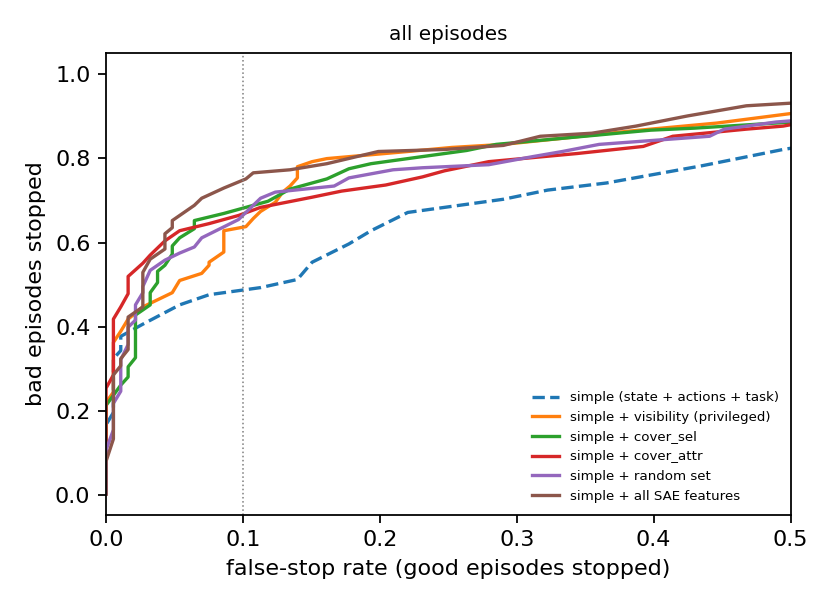
\includegraphics{../figures/fig_E7_stoprule.png}
\caption{stop rule}
\end{figure}

\emph{Figure 2. Fraction of bad episodes stopped as a function of the
fraction of good episodes stopped.}

\textbf{Hazard-level early warning} (will the event happen within 1.6
s?) shows the same pattern:

\begin{itemize}
\tightlist
\item
  For wrong-object lifting (61 events), AUPRC rises from 0.34 (state) to
  0.64 (+ selected features), 0.69 (+ random features) and 0.79 (+ all
  features). Median warning lead is 41--53 steps (about 2--2.7 s).
\item
  The number of harmless episodes that ever receive an alarm also rises,
  from 27\% to about 50\%.
\end{itemize}

\textbf{Take-away.} VLA activations carry actionable information about
impending harm that robot state lacks. A cheap monitor on them
intercepts most harms before they happen. The information is
\textbf{generic}: random features work as well as ``occlusion
features''. Interpretability adds no specific monitoring value here, and
we recommend random-feature controls as standard for such claims.

\hypertarget{can-the-internals-make-the-robot-more-careful}{%
\subsection{6. Can the internals make the robot more
careful?}\label{can-the-internals-make-the-robot-more-careful}}

We find transcoder features that predict future end-effector speed and
gripper closure on held-out episodes:

\begin{longtable}[]{@{}
  >{\raggedright\arraybackslash}p{(\columnwidth - 4\tabcolsep) * \real{0.3333}}
  >{\raggedright\arraybackslash}p{(\columnwidth - 4\tabcolsep) * \real{0.3333}}
  >{\raggedright\arraybackslash}p{(\columnwidth - 4\tabcolsep) * \real{0.3333}}@{}}
\toprule\noalign{}
\begin{minipage}[b]{\linewidth}\raggedright
Target
\end{minipage} & \begin{minipage}[b]{\linewidth}\raggedright
Features
\end{minipage} & \begin{minipage}[b]{\linewidth}\raggedright
Baselines
\end{minipage} \\
\midrule\noalign{}
\endhead
\bottomrule\noalign{}
\endlastfoot
speed & r = 0.73 (``fast'' set) / −0.79 (``slow'' set) & current speed r
= 0.41 \\
gripper close within 16 steps & AUROC 0.995 & proprioception 0.996 \\
\end{longtable}

Against the policy's \emph{already-planned} action chunk:

\begin{longtable}[]{@{}lll@{}}
\toprule\noalign{}
Target & Planned chunk & Features, given the plan \\
\midrule\noalign{}
\endhead
\bottomrule\noalign{}
\endlastfoot
speed & r = 0.92 & partial r = 0.45 \\
gripper & AUROC 0.97 & AUROC 0.965 on rows whose chunk has no close \\
\end{longtable}

So the features are partly re-encodings of what the policy has already
decided.

We compare three levers (5 tasks × 10 initial states per condition; 95\%
task-clustered CIs vs the unmodified policy):

\begin{longtable}[]{@{}
  >{\raggedright\arraybackslash}p{(\columnwidth - 6\tabcolsep) * \real{0.2500}}
  >{\raggedright\arraybackslash}p{(\columnwidth - 6\tabcolsep) * \real{0.2500}}
  >{\raggedright\arraybackslash}p{(\columnwidth - 6\tabcolsep) * \real{0.2500}}
  >{\raggedright\arraybackslash}p{(\columnwidth - 6\tabcolsep) * \real{0.2500}}@{}}
\toprule\noalign{}
\begin{minipage}[b]{\linewidth}\raggedright
Lever
\end{minipage} & \begin{minipage}[b]{\linewidth}\raggedright
Δ speed (m/s)
\end{minipage} & \begin{minipage}[b]{\linewidth}\raggedright
Δ success
\end{minipage} & \begin{minipage}[b]{\linewidth}\raggedright
Other safety-relevant change
\end{minipage} \\
\midrule\noalign{}
\endhead
\bottomrule\noalign{}
\endlastfoot
Prompt ``\ldots slowly and carefully'' & −0.006 {[}−0.011, −0.000{]}
(−3\%) & −0.02 {[}−0.12, 0.06{]} & max contact force +1.2 {[}0.5, 1.8{]}
N \\
Clamp ``slow'' features on & −0.000 {[}−0.007, 0.004{]} & +0.04 {[}0.00,
0.08{]} & --- \\
Ablate ``fast'' features & −0.001 {[}−0.004, 0.003{]} & 0.00 &
intervention ≈ 0.4\% of MLP output norm \\
Boost gripper features (vs random control) & --- & −0.02 & closes 1.0
{[}0.5, 1.6{]} steps earlier; max force +2.0 {[}0.3, 4.0{]} N \\
Scale actions × 0.5 & −0.097 {[}−0.106, −0.088{]} (−55\%) &
\textbf{−0.76 {[}−0.98, −0.52{]}} & grasp rate −0.66 \\
Under the box: prompt & −0.001 & +0.02 {[}−0.04, 0.08{]} & --- \\
Under the box: scale × 0.5 & −0.036 & −0.12 {[}−0.22, −0.02{]} (6/50 →
0/50) & max force −8.3 {[}−12.2, −5.2{]} N \\
\end{longtable}

\textbf{Take-away.}

\begin{itemize}
\tightlist
\item
  Decodable speed and gripper features are not control knobs.
\item
  Language-level caution is almost ignored by the policy.
\item
  Crude action scaling reduces contact forces only by making the robot
  fail. Under occlusion it lowers peak force by 8 N and success to zero.
\end{itemize}

A dose--response check with stronger clamps did not run (Section 8), so
the steering null holds only at the strengths tested.

\hypertarget{discussion}{%
\subsection{7. Discussion}\label{discussion}}

For this VLA, the safety-relevant use of internals is \textbf{detection,
not control}. Three lessons for safety evaluations of interpretability
methods:

\begin{enumerate}
\def\labelenumi{\arabic{enumi}.}
\tightlist
\item
  \textbf{Measure outcomes, not proxies.} High decoding accuracy (AUROC
  0.995 for gripper closure) coexisted with no useful steering effect.
  Faithful reconstruction (FVU 0.175) coexisted with no sparse causal
  handle.
\item
  \textbf{Always include random-feature and harmless-perturbation
  controls.} Without the random-feature stop rule we would have credited
  occlusion features with a +20-point safety gain that any feature set
  provides. Without the miss-box control we could not attribute the
  harms to lost target visibility.
\item
  \textbf{Pre-register the monitoring claim.} Our pre-registered test
  was negative even though several post-hoc views (step 0, held-out
  tasks, event precision) look positive. Reporting both avoids
  over-claiming.
\end{enumerate}

\hypertarget{limitations-and-gaps-before-submission}{%
\subsection{8. Limitations and gaps before
submission}\label{limitations-and-gaps-before-submission}}

\textbf{Limitations.}

\begin{itemize}
\tightlist
\item
  One policy and one simulated suite.
\item
  Occluders are synthetic, render-only boxes and panels.
\item
  5-task clusters in the repair and steering studies make those CIs
  coarse.
\item
  Transcoders were trained on all tasks, so leave-one-task-out holds
  tasks out of the monitor only.
\item
  The stop rule is an offline replay; a real stop changes what happens
  next.
\item
  ``Harm'' thresholds are our own definitions.
\end{itemize}

\textbf{Gaps, all {[}TODO before submission{]}.}

\begin{itemize}
\item
  \begin{enumerate}
  \def\labelenumi{(\roman{enumi})}
  \tightlist
  \item
    \textbf{Uncertainty baseline.} Disagreement across K sampled action
    chunks is the most natural non-interpretability monitor. It was
    implemented but did not run, because of a GPU runtime failure.
  \end{enumerate}
\item
  \begin{enumerate}
  \def\labelenumi{(\roman{enumi})}
  \setcounter{enumi}{1}
  \tightlist
  \item
    \textbf{Steering dose--response.} Also implemented; did not run for
    the same reason.
  \end{enumerate}
\item
  \begin{enumerate}
  \def\labelenumi{(\roman{enumi})}
  \setcounter{enumi}{2}
  \tightlist
  \item
    \textbf{Full monitoring analysis.} It was run in a reduced
    configuration: windows 0/48 instead of 0/24/48/80, C fixed at 0.1
    instead of a grid, 300 bootstraps instead of 1000, and 2
    random-feature draws evaluated instead of the planned 5. It should
    be re-run at full settings. The stop rule's random-feature
    comparison uses one draw (\texttt{rand\_cover\_sel\_0}).
  \end{enumerate}
\item
  \begin{enumerate}
  \def\labelenumi{(\roman{enumi})}
  \setcounter{enumi}{3}
  \tightlist
  \item
    \textbf{Citations.} Titles and authors of related work must be
    checked (references below are placeholders by identifier).
  \end{enumerate}
\end{itemize}

\hypertarget{references-to-be-completed}{%
\subsection{References (to be
completed)}\label{references-to-be-completed}}

\begin{itemize}
\tightlist
\item
  {[}Swann et al., arXiv:2603.19183{]} Sparse features of the pi0.5 VLM
  and steering. \textbf{TODO}: verify title and authors.
\item
  {[}OpenReview Ln0yjcSVku{]} VLA steering evaluated by task-completion
  speed, with a prompting control. \textbf{TODO}: verify.
\item
  {[}OpenReview ZVY1lSGcnZ{]} Action-expert activation probes predict
  task failure. \textbf{TODO}: verify.
\item
  {[}arXiv:2609.06326{]} \emph{Rethinking Safety for Generalist Robots}.
  \textbf{TODO}: verify authors.
\item
  LIBERO benchmark; pi0.5 / openpi; LeRobot; TopK sparse autoencoders /
  transcoders. \textbf{TODO}: add standard citations.
\end{itemize}

\begin{center}\rule{0.5\linewidth}{0.5pt}\end{center}

\hypertarget{appendix-a-additional-numbers}{%
\subsection{Appendix A: Additional
numbers}\label{appendix-a-additional-numbers}}

\begin{itemize}
\item
  \textbf{Closed-loop reproducibility.} Re-running the 540 v3
  closed-loop episodes gives identical outcomes and lengths (540/540).
\item
  \textbf{Contact-force sensitivity.}

  \begin{longtable}[]{@{}lllll@{}}
  \toprule\noalign{}
  Condition & \textgreater1 N & \textgreater5 N & \textgreater10 N &
  \textgreater20 N \\
  \midrule\noalign{}
  \endhead
  \bottomrule\noalign{}
  \endlastfoot
  clean & 0.24 & 0.24 & 0.18 & 0.02 \\
  miss box & 0.29 & 0.26 & 0.20 & 0.04 \\
  box & 0.67 & 0.65 & 0.51 & 0.19 \\
  static box & 0.63 & 0.62 & 0.50 & 0.14 \\
  screen & 0.50 & 0.47 & 0.43 & 0.17 \\
  \end{longtable}
\item
  \textbf{Within-condition failure prediction} (step 48, AUROC). Under
  the box itself the state baseline is best (0.79 vs 0.73 for the
  selected features). Under the screen the features are slightly better
  (0.83--0.87 vs 0.81).
\item
  \textbf{Unwanted-contact warnings (\textgreater1 N, 280 events).}
  AUROC 0.81 (state), 0.84 (+ selected), 0.86 (+ random), 0.88 (+ all
  features).
\item
  \textbf{Drop warnings (144 events).} AUROC 0.92 (state) vs 0.93--0.94
  with features. Episode false-alarm rates are high for every monitor
  (58--73\%).
\item
  \textbf{8192-feature dictionary, open loop, cover occluder.}
  Attribution top-K reproduces 0.2 / 1.0 / 10.8 / 19.5\% of the effect
  at K = 10 / 100 / 1000 / 3000. Oracle ranking reaches 4.3 / 16.0 /
  27.5 / 27.9\%. Random reaches 0.0 / −0.0 / 0.1 / 0.6\%. Selective and
  attribution sets share 3 of 100 features.
\end{itemize}

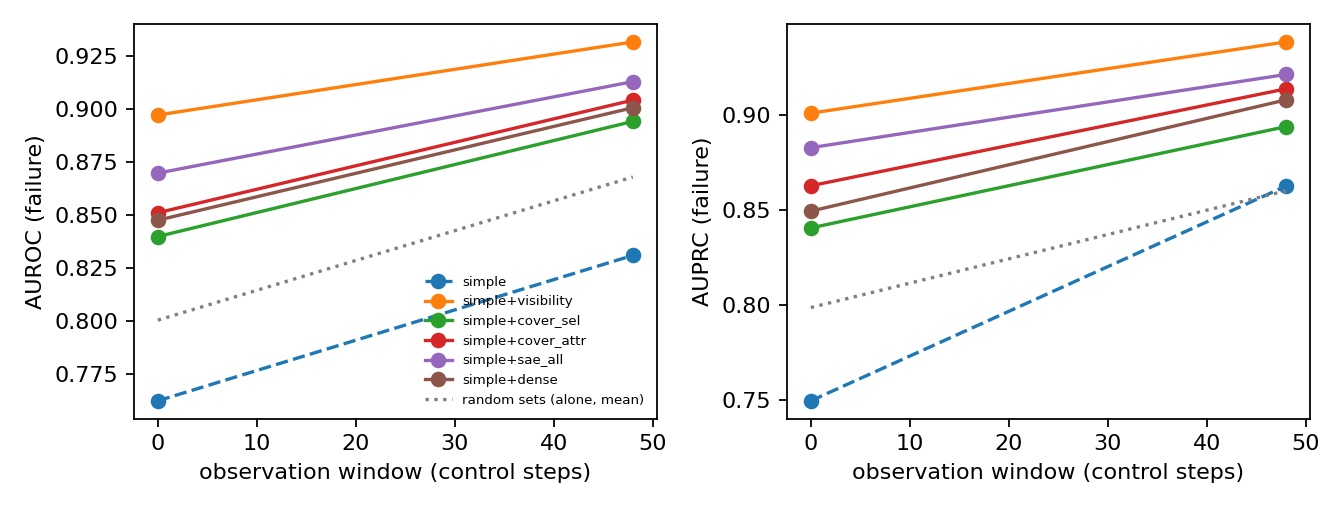
\includegraphics{../figures/fig_E3_monitor_windows.png}
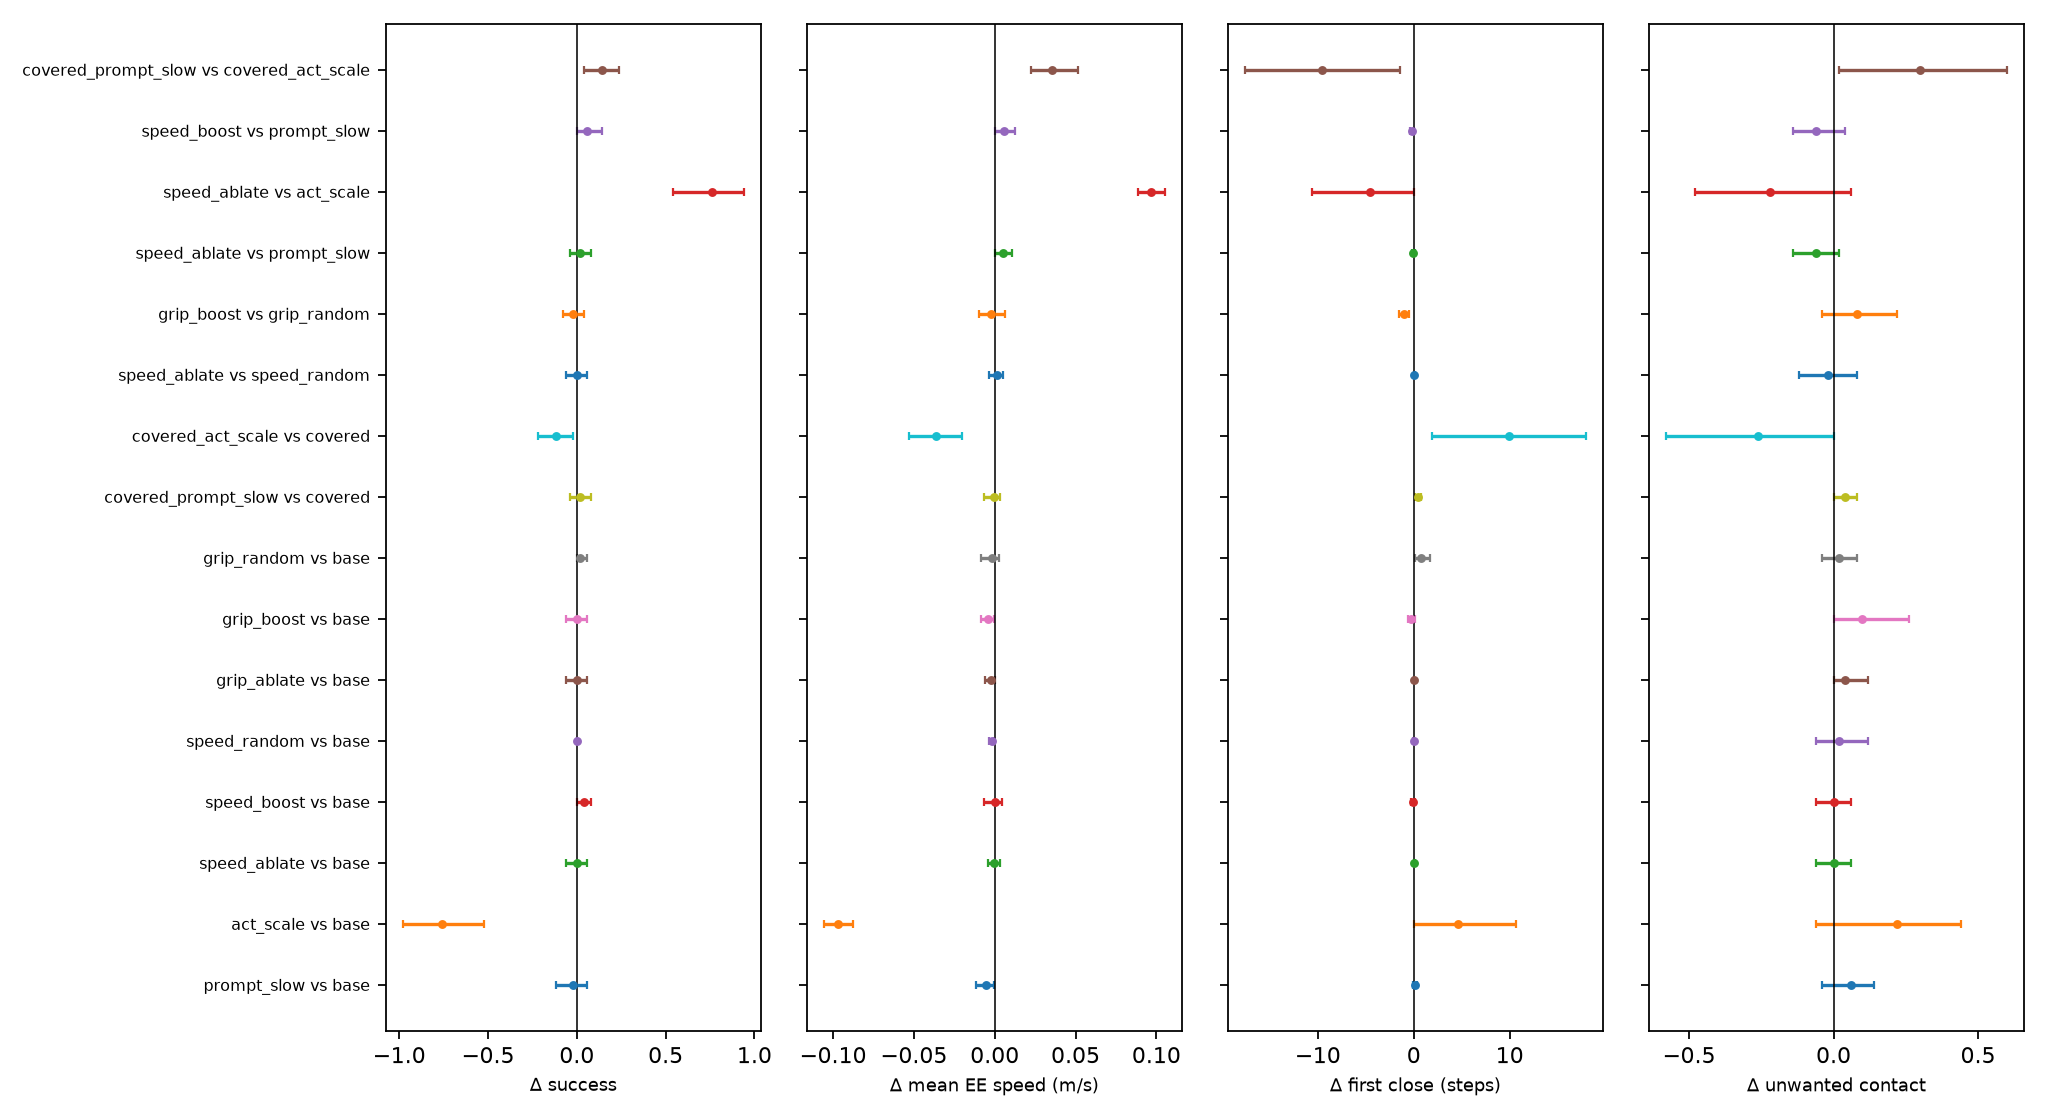
\includegraphics{../figures/fig_E5_steering_forest.png}
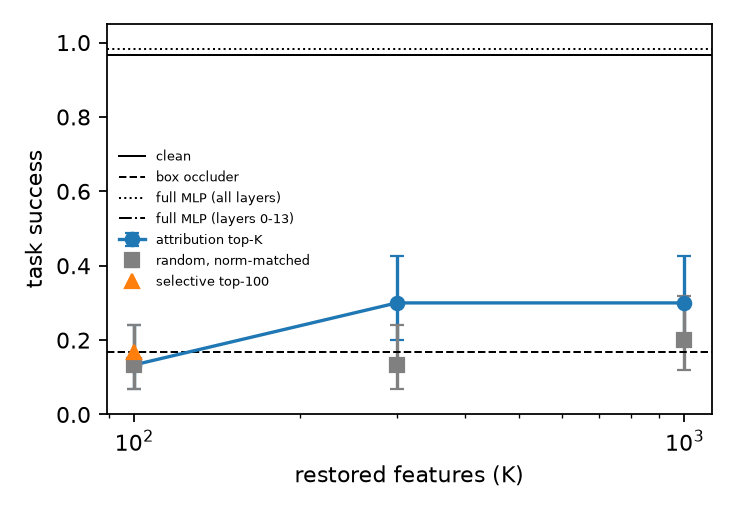
\includegraphics{../figures/fig_E2_dose.png}

\end{document}
